\documentclass{article}
\usepackage[T1]{fontenc}
\usepackage[latin1]{inputenc}
\usepackage[brazilian]{babel}

\title{Método dos Elementos Finitos e problemas de valor de contorno aplicados à Teoria Eletromagnética}
\author{Thiago de Sousa Goveia }
\date{16 de Janeiro de 2017}

\usepackage{natbib}
\usepackage{graphicx}
\usepackage{amsmath}

\begin{document}

\maketitle

\section{Problema de Valor de Contorno}

A solução de problemas envolvendo um modelo matemático descrito por uma equação ou sistema de equações diferenciais, pode ser obtida  a partir da especificação das condições iniciais ou das condições de contorno do domínio. Tais condições adicionais formalizam respectivamente, os problemas de valor inicial e de valor de contorno relacionados ao modelo em questão.

Para se definir um problema de valor inicial (PVI), dado um modelo de ordem N, é preciso estabelecer em um determinado ponto, os valores da variável dependente e de suas derivadas até a ordem N-1. Se alguma condição for dada em algum ponto diferente do primeiro, tem-se definido o problema de valor de contorno (PVC). Enquanto os PVI geralmente envolvem o tempo como variável independente, os PVC normalmente são definidos em função do espaço e representam a resposta em estado estacionário de um problema variante no tempo.
\citep[p. 447]{boyce_diprima}

Dado o domínio $ \Omega $ tal que

\begin{equation}
  \Omega \subset \Re^{n}
\end{equation}

Os valores na fronteira $ \partial \Omega $ do domínio são definidos por uma função $ u(x, y) $ tal que

\begin{equation}
  u(x, y) = f(x, y),  \forall (x, y) \in \partial \Omega
\end{equation}

Assim, conhecendo-se os valores na borda, é possível inferir o conjunto de funções em $ \Omega $ que seja solução do modelo. 

De forma a exemplificar, considere o caso simples, em que o domínio $ \Omega $ seja um intervalo aberto em $ \Re $ e os pontos da fronteira sejam os extremos deste intervalo: 

\begin{equation}
  [a, b] \subset \Re
\end{equation}

\begin{equation}
  \Omega = [a, b]
\end{equation}

\begin{equation}
  \partial [a, b] = \{ a, b \}
\end{equation}

Um problema de valor de contorno definido sobre este domínio é portanto, composto pela equação que modela o comportamento do processo e pelas condições adicionais de contorno


\begin{equation}
    \label{eq:pvc}
    PVC = 
    \begin{cases}
        y'' = f(x, y, y') \\
        y(a) = \alpha \\
        y(b) = \beta
    \end{cases}
\end{equation}

Conforme mostra a figura ~\ref{fig:pvc}, a solução para o exemplo dado, consiste em encontrar a curva ou o conjunto de curvas que obedeçam às condições de contorno.

\begin{figure}[ht!]
\centering
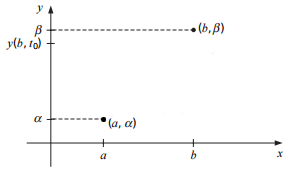
\includegraphics[scale=0.8]{figuras/PVC.png}
\caption{PVC: Encontrar a curva solução entre os pontos $ \alpha $ e $ \beta $}
\label{fig:pvc}
\end{figure}

\subsection{Métodos de resolução de PVC}
\subsubsection{Método do Chute}
O Método do chute consiste basicamente na substituição de um problema de valor de contorno por dois problemas de valor inicial. Para o caso de equações diferenciais ordinárias, com $ \Omega \subset \Re $ , o valor de  $ y(b) $ é obtido a partir da inclinação adequada da curva no ponto $ (a, \alpha) $. A figura ~\ref{fig:chute} ilustra este método.
\citep[p. 674]{burden_faires}


\begin{figure}[ht!]
\centering
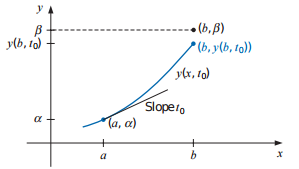
\includegraphics[scale=0.8]{figuras/Shooting.png}
\caption{Método do chute: o valor de $ \beta $ aproximado a partir da inclinação da derivada em $ (a, \alpha) $}
\label{fig:chute}
\end{figure}


\section{Método das diferenças finitas}

O método das diferenças finitas substitui cada derivada da equação diferencial por um quociente-diferença apropriado,
\citep[p. 684]{burden_faires}
isto é, obter aproximações discretas para cada derivada.

Sendo o domínio $ \Omega $ contínuo e limitado em $ x = {a, b} $, o mesmo pode ser discretizado escolhendo-se um valor $ N > 0 $ e dividindo-se o intervalo $ [a, b] $ em $ N + 1 $ subintervalos iguais, os quais são limitados por

\begin{equation}
  x_i = a + ih,  i = 0, 1, ... N+1
\end{equation}

O valor do incremento h é dado por 

\begin{equation}
  h = \frac{b-a}{N+1}
\end{equation}

Nos pontos interiores $ x_i , com i = 1, 2. .... N $, isto é, dentro da borda $ {a, b} $, a equação diferencial a ser aproximada é

\begin{equation}
    \label{eq:edo2}
    y''(x_i) = p(x_i)y'(x_i) + q(x_i)y(x_i) + r(x_i)
\end{equation}

Deseja-se obter o valor de $ y(x_i) $ como uma média do valor de seus vizinhos $ y(x_i + h) $ e $ y(x_i - h) $. Para tal, utiliza-se a expansão em série de Taylor, como por exemplo, a de ordem 3. A notação do grande O foi utilizada para denotar o erro do truncamento.

\begin{equation}
    \label{eq:dfr}
    y(x_i + h) = y(x_i) + hy'(x_i) + \frac{h^{2}}{2}y''(x_i) + \frac{h^{3}}{6}y'''(x_i) + O(h^{4})
\end{equation}

\begin{equation}
    \label{eq:dfl}
    y(x_i - h) = y(x_i) - hy'(x_i) + \frac{h^{2}}{2}y''(x_i) - \frac{h^{3}}{6}y'''(x_i) + O(h^{4})
\end{equation}

Somando-se as equações \ref{eq:dfr} e \ref{eq:dfl} e isolando a derivada procurada, no caso a de segunda ordem.

\begin{equation}
    \label{eq:difcent2}
    y''(x_i) = \frac{1}{h^2}[y(x_i + h) - 2y(x_i) +y(x_i - h)] - O(h^{4})
\end{equation}

A equação \ref{eq:difcent2} é denomidada fórmula da diferença centrada, pois obtém o valor de um dado ponto a partir do valor de todos os seus vizinhos. De forma similar, para a derivada de primeira ordem, obtém-se

\begin{equation}
    \label{eq:difcent}
    y'(x_i) = \frac{1}{2h}[y(x_i + h) - y(x_i - h)] - O(h^{2})
\end{equation}

Com as derivadas da equação \ref{eq:edo2} definidas, obtém-se então a sua forma discretizada. Os termos de ordem superior relativos ao erro de aproximação, foram desconsiderados na equação \ref{eq:edoDisc}.

\begin{equation}
    \label{eq:edoDisc}
   \frac{y(x_i + h) - 2y(x_i) +y(x_i - h)}{h^2} = p(x_i) \frac{y(x_i + h) - y(x_i - h)}{2h} +q(x_i)y(x_i) + r(x_i)
\end{equation}


O resultado obtido em  \ref{eq:edoDisc} pode ser expandido para M dimensões. As equações \ref{eq:lap} e \ref{eq:lapDisc} mostram a equação de laplace em duas dimensões e a mesma equação discretizada.

\begin{equation}
    \label{eq:lap}
    \Delta u = \frac{\partial^2 u}{\partial^2 x} + \frac{\partial^2 u}{\partial^2 y} = 0
\end{equation}

\begin{equation}
    \label{eq:lapDisc}
   \frac{u(x + h, y) - 2u(x, y) +u(x - h, y)}{h^2} +
   \frac{u(x, y + h) - 2u(x, y) +u(x, y - )}{h^2} = 0
\end{equation}
\subsection{Condições de Contorno}

\subsubsection{Condição de Dirichlet}

\subsubsection{Condição de Neumann}

\subsubsection{Condição Mista}

\subsubsection{Condição Sturm-Liouville}
\section{Método dos Elementos Finitos}

Muitos problemas de valor de contorno não podem ser resolvidos por métodos analíticos, uma vez que surgem dificuldades ao lidar com características específicas do modelo, tais como coeficientes variáveis, regiões irregulares, condições de contorno inadequadas, existência de interfaces ou a grande quantidade de detalhes.
\citep{powers}


\bibliographystyle{plain}
\bibliography{references}
\end{document}
